%Este trabalho está licenciado sob a Licença Atribuição-CompartilhaIgual 4.0 Internacional Creative Commons. Para visualizar uma cópia desta licença, visite http://creativecommons.org/licenses/by-sa/4.0/deed.pt_BR ou mande uma carta para Creative Commons, PO Box 1866, Mountain View, CA 94042, USA.

\chapter{Perceptron Multicamadas}\label{cap_mlp}
\thispagestyle{fancy}

\section{Modelo MLP}\label{cap_mlp_sec_modelo}

\hl{Uma Perceptron Multicamadas (MLP, do inglês, \textit{Multilayer Perceptron}) é um tipo de Rede Neural Artificial formada por composições de camadas de perceptrons}. Consulte a Figura \ref{cap_mlp_sec_modelo}.

\begin{figure}[H]
  \centering
  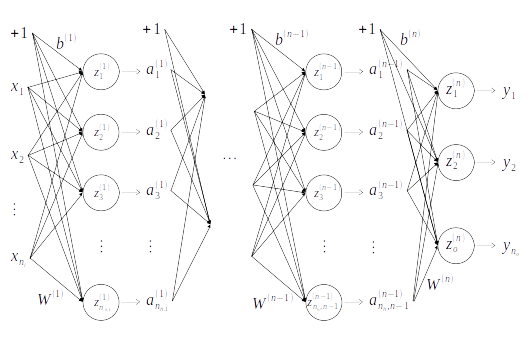
\includegraphics[width=\textwidth]{./cap_mlp/dados/fig_mlp/fig}
  \caption{Estrutura de uma rede do tipo Perceptron Multicamadas (MLP).}
  \label{fig:cap_mlp_sec_modelo:fig:mlp}
\end{figure}

\hl{Denotamos uma MLP de $n$ camadas por}
\begin{equation}\hleq
  \pmb{y} = \mathcal{N}\left(\pmb{x}; \left(W^{(l)}, \pmb{b}^{(l)}, f^{(l)}\right)_{l=1}^{n}\right),
\end{equation}
onde $\left(W^{(l)}, \pmb{b}^{(l)}, f^{(l)}\right)$ é a tripa de \emph{pesos}, \emph{\textit{biases}} e \emph{função de ativação} da $l$-ésima camada da rede, $l=1, 2, \dotsc, n$.

\hl{A saída da rede é calculada por iteradas composições das camadas}, i.e.
\begin{equation}\hleq
  \pmb{a}^{(l)} = f^{(l)}\underbrace{\left(W^{(l)}\pmb{a}^{(l-1)} + \pmb{b}^{(l-1)}\right)}_{\pmb{z}^{(l)}},
\end{equation}
para $l= 1, 2, \dotsc, n$, denotando $\pmb{a}^{(0)} := \pmb{x}$ e $\pmb{a}^{(n)} := \pmb{y}$.

\subsection{Treinamento}\label{cap_mlp_sec_modelo:ssec:treinamento}

Fornecido um \emph{conjunto de treinamento} $\{\pmb{x}^{(s)}, \pmb{y}^{(s)}\}_{s=1}^{n_s}$, com $n_s$ amostras, \hl{o treinamento da rede consiste em resolver o problema de minimização}
\begin{equation}\hleq
  \min_{(W,\pmb{b})}\varepsilon\left(\tilde{\pmb{y}}^{(s)}, \pmb{y}^{(s)}\right)
\end{equation}
onde $\varepsilon$ é uma dada \emph{função erro} (em inglês, \textit{loss function}) e $\tilde{\pmb{y}}^{(s)}$, $\pmb{y}^{(s)}$ são as saídas estimada e esperada da $l$-ésima amostra, respectivamente.

\hl{O problema de minimização pode ser resolvido por um }\href{https://notaspedrok.com.br/notas/MatematicaNumericaAvancada/cap\_otimizacao_sec_minimi.html}{\hl{Método de Declive}} e, de forma geral, consiste em:
\begin{enumerate}
\item $W, \pmb{b}$ aproximações iniciais.
\item Para $e\leftarrow 1, \dotsc, n_e$:
  \begin{enumerate}\hleq
  \item $\displaystyle (W, \pmb{b}) \leftarrow (W, \pmb{b}) - l_r\pmb{d}\left(\nabla_{W,\pmb{b}} \varepsilon\right)$
  \end{enumerate}
\end{enumerate}
onde, $n_e$ é o \emph{número de épocas}, $l_r$ é uma dada \emph{taxa de aprendizagem} (em inglês, \textit{learning rate})) e o vetor direção $\pmb{d} = \pmb{d}\left(\nabla_{W,\pmb{b}} \varepsilon\right)$, onde
\begin{equation}\hleq
  \nabla_{W,\pmb{b}} \varepsilon := \left(\frac{\p\varepsilon}{\p W}, \frac{\p\varepsilon}{\p\pmb{b}}\right).
\end{equation}

\hl{O cálculo dos gradientes pode ser feito \emph{de trás para frente}} (em inglês, \textit{backward}), i.e. para os pesos da última camada, temos
\begin{align}
  \hleq{\frac{\p\varepsilon}{\p W^{(n)}}} &\hleq{= \frac{\p\varepsilon}{\p\pmb{y}}\frac{\p\pmb{y}}{\p\pmb{z^{(n)}}}\frac{\p\pmb{z^{(n)}}}{\p W^{(n)}}},\\
                             &= \frac{\p\varepsilon}{\p\pmb{y}}f'\left(W^{(n)}\pmb{a}^{(n-1)}+\pmb{b}^{(n)}\right)\pmb{a}^{(n-1)}.
\end{align}
Para os pesos da penúltima, temos
\begin{align}
  \hleq{\frac{\p\varepsilon}{\p W^{(n-1)}}} &\hleq{= \frac{\p\varepsilon}{\p\pmb{y}}\frac{\p\pmb{y}}{\p\pmb{z^{(n)}}}\frac{\p\pmb{z^{(n)}}}{\p W^{(n-1)}}},\\
                                     &= \frac{\p\varepsilon}{\p\pmb{y}}f'\left(\pmb{z}^{(n)}\right)\frac{\p\pmb{z}^{(n)}}{\p\pmb{a}^{(n-1)}}\frac{\p\pmb{a}^{(n-1)}}{\p\pmb{z}^{(n-1)}}\frac{\p\pmb{z}^{(n-1)}}{\p W^{(n-1)}}\\
                                     &= \frac{\p\varepsilon}{\p\pmb{y}}f'\left(\pmb{z}^{(n)}\right)W^{(n)}f'\left(\pmb{z}^{(n-1)}\right)\pmb{a}^{(n-2)}
\end{align}
e assim, sucessivamente para as demais camadas da rede. \hl{Os gradientes em relação aos \textit{biases} podem ser analogamente calculados}.

\subsection{Aplicação: Problema de Classificação \texttt{XOR}}

Vamos desenvolver uma MLP que faça a operação $\texttt{xor}$ (ou exclusivo). I.e, receba como entrada dois valores lógicos $A_1$ e $A_2$ (V, verdadeiro ou F, falso) e forneça como saída o valor lógico $R = A_1 \texttt{xor} A_2$. Consultamos a seguinte tabela verdade:

\begin{center}
  \begin{tabular}{cc|c}
    $A_1$ & $A_2$ & $R$\\\hline
    V & V & F\\
    V & F & V\\
    F & V & V\\
    F & F & F\\\hline
  \end{tabular}
\end{center}

Assumindo $V = 1$ e $F = -1$, podemos modelar o problema tendo entradas $\pmb{x} = (x_1, x_2)$ e saída $y$ como na seguinte tabela:

\begin{center}
  \begin{tabular}{rr|r}
    $x_1$ & $x_2$ & $y$ \\\hline
    $1$ & $1$ & $-1$ \\
    $1$ & $-1$ & $1$ \\
    $-1$ & $1$ & $1$ \\
    $-1$ & $-1$ & $-1$ \\\hline
  \end{tabular}
\end{center}

\subsubsection{Modelo}

Vamos usar uma MLP de estrutura $2-2-1$ e com funções de ativação $f^{(1)}(\pmb{x}) = \tanh(\pmb{x})$ e $f^{(2)}(\pmb{x}) = id(\pmb{x})$. Ou seja, nossa rede tem duas entradas, uma \emph{camada escondida} com 2 unidades (função de ativação tangente hiperbólica) e uma camada de saída com uma unidade (função de ativação identidade).

\subsubsection{Treinamento}

Para o treinamento, vamos usar a função \hl{\emph{erro quadrático médio}} (em inglês, \textit{mean squared error})
\begin{equation}\hleq
  \varepsilon := \frac{1}{n_s}\sum_{s=1}^{n_s}\left|\tilde{y}^{(s)} - y^{(s)}\right|^2,
\end{equation}
onde os valores estimados $\tilde{y}^{(s)} = \mathcal{N}\left(\pmb{x}^{(s)}\right)$ e $\left\{\pmb{x}^{(s)}, y^{(s)}\right\}_{s=1}^{n_s}$, $n_s=4$, conforme na tabela acima.

\subsubsection{Implementação}

O seguinte código implementa a MLP e usa o \hl{Método do Gradiente Descendente (DG) no algoritmo de treinamento}.

% \lstinputlisting[caption=mlp\_xor.py, label=cap_mlp_sec_modelo:cod:mlp_xor]{./cap_mlp/dados/py_mlp_xor/main.py}
\begin{lstlisting}[caption=mlp\_xor.py, label=cap_mlp_sec_modelo:cod:mlp_xor]
import torch

# modelo

model = torch.nn.Sequential(
    torch.nn.Linear(2,2),
    torch.nn.Tanh(),
    torch.nn.Linear(2,1)
    )

# treinamento

## optimizador
optim = torch.optim.SGD(model.parameters(), lr=1e-2)

## função erro
loss_fun = torch.nn.MSELoss()

## dados de treinamento
X_train = torch.tensor([[1., 1.],
                  [1., -1.],
                  [-1., 1.],
                  [-1., -1.]])
y_train = torch.tensor([-1., 1., 1., -1.]).reshape(-1,1)

print("\nDados de treinamento")
print("X_train =")
print(X_train)
print("y_train = ")
print(y_train)

## num max épocas
nepochs = 5000
tol = 1e-3

for epoch in range(nepochs):

    # forward
    y_est = model(X_train)

    # erro
    loss = loss_fun(y_est, y_train)

    print(f'{epoch}: {loss.item():.4e}')

    # critério de parada
    if (loss.item() < tol):
        break

    # backward
    optim.zero_grad()
    loss.backward()
    optim.step()


# verificação
y = model(X_train)
print(f'y_est = {y}')
\end{lstlisting}

\subsection{Exercícios}

[[tag::construcao]]

\section{Aplicação: Problema de Classificação Binária}\label{cap_mlp_sec_classbin}

Vamos estudar uma aplicação de redes neurais artificiais em um problema de classificação binária não linear.

\subsection{Dados}

Vamos desenvolver uma rede do tipo Perceptron Multicamadas (MLP) para a classificação binária de pontos, com base nos seguintes dados.

\begin{lstlisting}
from sklearn.datasets import make_circles
import matplotlib.pyplot as plt

plt.rcParams.update({
     "text.usetex": True,
     "font.family": "serif",
     "font.size": 14
     })

# data
print('data')
n_samples = 1000
print(f'n_samples = {n_samples}')
# X = points, y = labels
X, y = make_circles(n_samples,
                    noise=0.03, # add noise
                    random_state=42) # random seed

fig = plt.figure()
ax = fig.add_subplot()
ax.scatter(X[:,0], X[:,1], c=y, cmap=plt.cm.coolwarm)
ax.grid()
ax.set_xlabel('$x_1$')
ax.set_ylabel('$x_2$')
plt.show()
\end{lstlisting}

\begin{figure}[H]
  \centering
  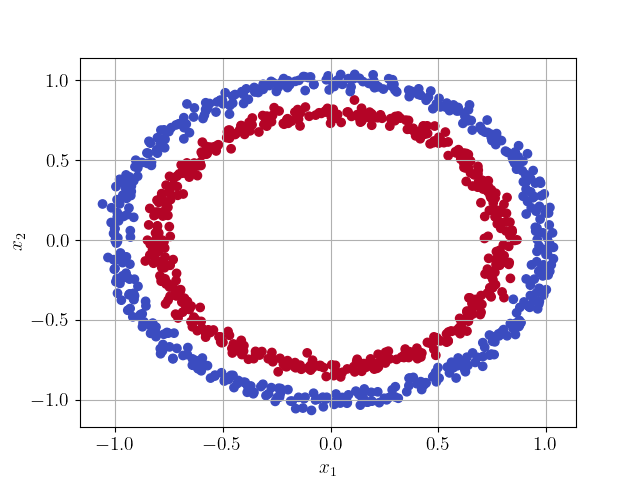
\includegraphics[width=0.8\textwidth]{./cap_mlp/dados/fig_classbin/fig}
  \caption{Dados para a o problema de classificação binária não linear.}
  \label{cap_mlp_sec_classbin:fig:dados}
\end{figure}

\subsection{Modelo}

Vamos usar uma MLP de estrutura 2-10-1, com função de ativação
\begin{equation}
  \elu(x) = \left\{
    \begin{array}{ll}
      x &, x > 0\\
      \alpha\left(e^x - 1\right) &, x \leq 0
    \end{array}
\right.
\end{equation}
na camada escondida e
\begin{equation}
  \sigmoid(x) = \frac{1}{1 + e^x}
\end{equation}
na saída da rede.

Para o treinamento e teste, vamos randomicamente separar os dados em um conjunto de treinamento $\{\pmb{x}_{\text{train}}^{(k)}, y_{\text{train}}^{(k)}\}_{k=1}^{n_{\text{train}}}$ e um conjunto de teste $\{\pmb{x}_{\text{test}}^{(k)}, y_{\text{test}}^{(k)}\}_{k=1}^{n_{\text{test}}}$, com $y=0$ para os pontos azuis e $y=1$ para os pontos vermelhos.

\subsection{Treinamento e Teste}

\begin{lstlisting}[caption=mlp\_classbin.py, label=cap_mlp_sec_classbin:cod:classbin]
import torch
from sklearn.datasets import make_circles
from sklearn.model_selection import train_test_split
import matplotlib.pyplot as plt

# data
print('data')
n_samples = 1000
print(f'n_samples = {n_samples}')
# X = points, y = labels
X, y = make_circles(n_samples,
                    noise=0.03, # add noise
                    random_state=42) # random seed

## numpy -> torch
X = torch.from_numpy(X).type(torch.float)
y = torch.from_numpy(y).type(torch.float).reshape(-1,1)

## split into train and test datasets
print('Data: train and test sets')
X_train, X_test, y_train, y_test = train_test_split(X,
                                                    y,
                                                    test_size=0.2,
                                                    random_state=42)
print(f'n_train = {len(X_train)}')
print(f'n_test = {len(X_test)}')
plt.close()
plt.scatter(X_train[:,0], X_train[:,1], c=y_train,
            marker='o', cmap=plt.cm.coolwarm, alpha=0.3)
plt.scatter(X_test[:,0], X_test[:,1], c=y_test,
            marker='*', cmap=plt.cm.coolwarm)
plt.show()

# model
model = torch.nn.Sequential(
    torch.nn.Linear(2, 10),
    torch.nn.ELU(),
    torch.nn.Linear(10, 1),
    torch.nn.Sigmoid()
    )

# loss fun
loss_fun = torch.nn.BCELoss()

# optimizer
optimizer = torch.optim.SGD(model.parameters(),
                            lr = 1e-1)

# evaluation metric
def accuracy_fun(y_pred, y_exp):
    correct = torch.eq(y_pred, y_exp).sum().item()
    acc = correct/len(y_exp) * 100
    return acc

# train
n_epochs = 10000
n_out = 100

for epoch in range(n_epochs):
    model.train()

    y_pred = model(X_train)

    loss = loss_fun(y_pred, y_train)

    acc = accuracy_fun(torch.round(y_pred),
                       y_train)

    optimizer.zero_grad()
    loss.backward()
    optimizer.step()

    model.eval()

    #testing
    if ((epoch+1) % n_out == 0):
        with torch.inference_mode():
            y_pred_test = model(X_test)
            loss_test = loss_fun(y_pred_test,
                                 y_test)
            acc_test = accuracy_fun(torch.round(y_pred_test),
                                    y_test)

        print(f'{epoch+1}: loss = {loss:.5e}, accuracy = {acc:.2f}%')
        print(f'\ttest: loss = {loss:.5e}, accuracy = {acc:.2f}%\n')
\end{lstlisting}

\subsection{Verificação}

Para a verificação, testamos o modelo em uma malha uniforme de $100\times 100$ pontos no domínio $[-1, 1]^2$. Consulte a Figure \ref{cap_mlp_sec_classbin:fig:result}.

\begin{figure}[H]
  \centering
  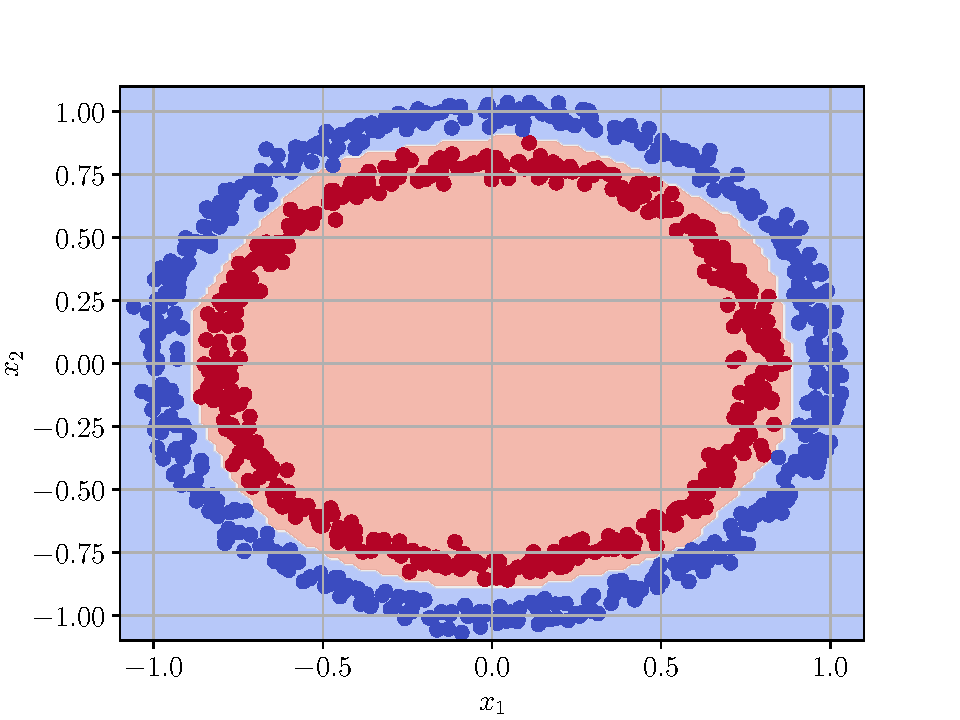
\includegraphics[width=0.8\textwidth]{./cap_mlp/dados/fig_classbin_result/fig}
  \caption{Verificação do modelo de classificação binária.}
  \label{cap_mlp_sec_classbin:fig:result}
\end{figure}


\begin{lstlisting}
# malha de pontos
xx = torch.linspace(-1.1, 1.1, 100)
Xg, Yg = torch.meshgrid(xx, xx)

# valores estimados
Zg = torch.empty_like(Xg)
for i,xg in enumerate(xx):
    for j,yg in enumerate(xx):
        z = model(torch.tensor([[xg, yg]])).detach()
        Zg[i, j] = torch.round(z)

# visualização
fig = plt.figure()
ax = fig.add_subplot()
ax.contourf(Xg, Yg, Zg, levels=2, cmap=plt.cm.coolwarm, alpha=0.5)
ax.scatter(X[:,0], X[:,1], c=y, cmap=plt.cm.coolwarm)
plt.show()
\end{lstlisting}

\subsection{Exercícios}

[[tag:construcao]]


\section{Aplicação: Aproximação de Funções}\label{cap_mlp_sec_apfun}

\hl{Redes Perceptron Multicamadas (MLP) são aproximadoras universais}. Nesta seção, vamos aplicá-las na aproximação de funções uni- e bidimensionais.

\subsection{Função unidimensional}

Vamos criar uma MLP para aproximar a função gaussiana
\begin{equation}
  y = e^{-x^2},
\end{equation}
para $x\in [-1,1]$.

% \lstinputlisting[caption=mlp\_gaussiana\_1d.py, label=cap_mlp_sec_modelo:cod:mlp_gaussiana_1d]{./cap_mlp/dados/py_mlp_gaussiana_1d/main.py}
\begin{lstlisting}
import torch
import matplotlib.pyplot as plt

# modelo

model = torch.nn.Sequential(
    torch.nn.Linear(1,25),
    torch.nn.Tanh(),
    torch.nn.Linear(25,1)
    )

# treinamento

## fun obj
fobj = lambda x: torch.exp(-x**2)
a = -1.
b = 1.

## optimizador
optim = torch.optim.SGD(model.parameters(),
                        lr=1e-2, momentum=0.9)

## função erro
loss_fun = torch.nn.MSELoss()

## num de amostras por época
ns = 100
## num max épocas
nepochs = 5000
## tolerância
tol = 1e-5

for epoch in range(nepochs):

    # amostras
    X_train = (a - b) * torch.rand((ns,1)) + b
    y_train = fobj(X_train)
    
    # forward
    y_est = model(X_train)

    # erro
    loss = loss_fun(y_est, y_train)

    print(f'{epoch}: {loss.item():.4e}')

    # critério de parada
    if (loss.item() < tol):
        break

    # backward
    optim.zero_grad()
    loss.backward()
    optim.step()


# verificação
fig = plt.figure()
ax = fig.add_subplot()

x = torch.linspace(a, b,
                   steps=50).reshape(-1,1)

y_esp = fobj(x)
ax.plot(x, y_esp, label='fobj')

y_est = model(x)
ax.plot(x, y_est.detach(), label='model')

ax.legend()
ax.grid()
ax.set_xlabel('x')
ax.set_ylabel('y')
plt.show()
\end{lstlisting}

\subsection{Função bidimensional}

Vamos criar uma MLP para aproximar a função gaussiana
\begin{equation}
  y = e^{-(x_1^2 + x_2^2)},
\end{equation}
para $\pmb{x} = (x_1, x_2)\in [-1,1]^2$.

% \lstinputlisting[caption=mlp\_gaussiana\_2d.py, label=cap_mlp_sec_modelo:cod:mlp_gaussiana_2d]{./cap_mlp/dados/py_mlp_gaussiana_2d/main.py}
\begin{lstlisting}
import torch
import matplotlib.pyplot as plt

# modelo

model = torch.nn.Sequential(
    torch.nn.Linear(2,50),
    torch.nn.Tanh(),
    torch.nn.Linear(50,25),
    torch.nn.Tanh(),
    torch.nn.Linear(25,5),
    torch.nn.Tanh(),
    torch.nn.Linear(5,1)
    )

# treinamento

## fun obj
a = -1.
b = 1.
def fobj(x):
    y = torch.exp(-x[:,0]**2 - x[:,1]**2)
    return y.reshape(-1,1)

## optimizador
optim = torch.optim.SGD(model.parameters(),
                        lr=1e-1, momentum=0.9)

## função erro
loss_fun = torch.nn.MSELoss()

## num de amostras por eixo por época
ns = 100
## num max épocas
nepochs = 5000
## tolerância
tol = 1e-5

for epoch in range(nepochs):

    # amostras
    x0 = (a - b) * torch.rand(ns) + b
    x1 = (a - b) * torch.rand(ns) + b
    X0, X1 = torch.meshgrid(x0, x1)
    X_train = torch.cat((X0.reshape(-1,1),
                         X1.reshape(-1,1)),
                        dim=1)
    y_train = fobj(X_train)
    
    # forward
    y_est = model(X_train)

    # erro
    loss = loss_fun(y_est, y_train)

    print(f'{epoch}: {loss.item():.4e}')

    # critério de parada
    if (loss.item() < tol):
        break

    # backward
    optim.zero_grad()
    loss.backward()
    optim.step()


# verificação
fig = plt.figure()
ax = fig.add_subplot()

n = 50
x0 = torch.linspace(a, b, steps=n)
x1 = torch.linspace(a, b, steps=n)
X0, X1 = torch.meshgrid(x0, x1)
X = torch.cat((X0.reshape(-1,1),
               X1.reshape(-1,1)),
              dim=1)

y_esp = fobj(X)
Y = y_esp.reshape((n,n))
levels = torch.linspace(0., 1., 10)
c = ax.contour(X0, X1, Y, levels=levels, colors='white')
ax.clabel(c)

y_est = model(X)
Y = y_est.reshape((n,n))
ax.contourf(X0, X1, Y.detach(), levels=levels)

ax.grid()
ax.set_xlabel('x_1')
ax.set_ylabel('x_2')
plt.show()
\end{lstlisting}

\subsection{Exercícios}

[[tag::construcao]]

\section{Diferenciação Automática}\label{cap_mlp_sec_autograd}

Uma RNA é uma composição de funções definidas por parâmetros (pesos e \textit{biases}). O treinamento de uma RNA ocorre em duas etapas\footnote{Para mais detalhes, consulte a Subseção \ref{cap_mlp_sec_modelo:ssec:treinamento}.}:
\begin{enumerate}[1.]
\item \hl{\emph{Propagação (\textit{forward})}}: os dados de entrada são propagados para todas as funções da rede, produzindo a saída estimada.
\item \hl{\emph{Retropropagação (\textit{backward})}}: a computação do gradiente do erro\footnote{Medida da diferença entre o valor estimado e o valor esperado.} em relação aos parâmetros da rede é realizado coletando as derivadas (gradientes) das funções da rede. Pela regra da cadeia, essa coleta é feita a partir da camada de saída em direção a camada de entrada da rede.
\end{enumerate}

A \hl{Diferenciação Automática (\emph{Autograd}, do inglês, \textit{Automatic Gradient}) consiste na computação de derivadas a partir da regra da cadeia em uma estrutura computacional composta de funções elementares}. Esse é o caso \hl{em RNAs, a computação do gradiente da saída da rede em relação a sua entrada pode ser feita de forma similar à computação do gradiente do erro em relação aos seus parâmetros}.

\subsection{Autograd Perceptron}

Para um Perceptron\footnote{Consulte o Capítulo \ref{cap_perceptron} para mais informações sobre o Perceptron.}
\begin{subequations}
  \begin{align}
    \tilde{y} &= \mathcal{N}\left(\pmb{x}, (\pmb{w}, b)\right)\\
              &= f\underbrace{(\pmb{w}\cdot\pmb{x} + b)}_{z}
  \end{align}
\end{subequations}
temos que o gradiente da saída $y$ em relação à entrada $\pmb{x}$ pode ser computada como segue
\begin{subequations}
  \begin{align}
    \frac{\p \tilde{y}}{\p\pmb{x}} &= \frac{\p f}{\p z}\frac{\p z}{\p\pmb{x}}\\
                                   &= f'(z)\pmb{w}
  \end{align}
\end{subequations}

\begin{ex}
  Vamos treinar um Perceptron com função de ativação $f(z) = z$
  \begin{subequations}
    \begin{align}
      \tilde{y} &= \mathcal{N}(x; (w,b))\\
                &= wx + b
    \end{align}
  \end{subequations}
  que se ajusta ao conjunto de pontos\footnote{Consulte o Exercício \ref{cap_perceptron_sec_train:exer:ajuste}.}
  \begin{center}
    \begin{tabular}{l|ll}
      s & $x^{(s)}$ & $y^{(s)}$\\\hline
      1 & 0.5 & 1.2\\
      2 & 1.0 & 2.1\\
      3 & 1.5 & 2.6\\
      4 & 2.0 & 3.6\\\hline
    \end{tabular}
  \end{center}
  Uma vez treinado com função erro MSE\footnote{MSE, Erro Quadrático Médio.}, espera-se que o Perceptron corresponda a reta de mínimos quadrados\footnote{Para mais informações sobre essa aplicação, consulte a Subseção \ref{cap_perceptron_sec_unit:ssec:regr}.}
  \begin{equation}
    y = 1.54x + 0.45
  \end{equation}
  Portanto, espera-se que
  \begin{equation}
    \frac{\p \tilde{y}}{\p x} = 1.54.
  \end{equation}

\begin{lstlisting}[caption=autograd\_percep.py]
import torch

# modelo
model = torch.nn.Linear(1,1)

# treinamento

## optimizador
optim = torch.optim.SGD(model.parameters(),
                        lr=1e-1)

## função erro
loss_fun = torch.nn.MSELoss()

## dados de treinamento
X_train = torch.tensor([[0.5],
                        [1.0],
                        [1.5],
                        [2.0]])
y_train = torch.tensor([[1.2],
                        [2.1],
                        [2.6],
                        [3.6]])

## num max épocas
nepochs = 5000
nstop = 10

cstop = 0
loss_min = torch.finfo().max
for epoch in range(nepochs):

    # forward
    y_est = model(X_train)

    # erro
    loss = loss_fun(y_est, y_train)

    # critério de parada
    if (loss.item() >= loss_min):
        cstop += 1
    else:
        loss_min = loss.item()
        cstop = 0

    print(f'{epoch}: {loss.item():.4e}, '\
          + f'cstop = {cstop}/{nstop}')

    if (cstop == nstop):
        break

    # backward
    optim.zero_grad()
    loss.backward()
    optim.step()


# verificação
print(f'w = {model.weight}')
print(f'b = {model.bias}')

# autograd dy/dx

## forward
x = torch.tensor([[1.]],
                 requires_grad=True)
y = model(x)

## backward
y.backward()
dydx = x.grad
print(f'dy/dx = {dydx}')
\end{lstlisting}
\end{ex}

\subsection{Autograd MLP}

Os conceitos de diferenciação automática (\emph{autograd}) são diretamente estendidos para redes do tipo Perceptron Multicamadas (MLP, do inglês, \textit{Multilayer Perceptron}). No seguinte exemplo, exploramos o fato de MLPs serem aproximadoras universais e avaliamos a derivada de uma MLP na aproximação de uma função.

\begin{ex}\label{cap_mlp_sec_autograd:ex:fun1d}
  Vamos criar uma MLP
  \begin{equation}
    \tilde{y} = \mathcal{N}\left(x; \left(W^{(l)}, \pmb{b}^{(l)}, f^{(l)}\right)_{l=1}^{n}\right),
  \end{equation}
  que aproxima a função $y = \sen(\pi x)$ para $x\in [-1, 1]$
  
\begin{lstlisting}[caption=autograd\_fun1d.py]
import torch
import matplotlib.pyplot as plt

# modelo

model = torch.nn.Sequential(
    torch.nn.Linear(1,50),
    torch.nn.Tanh(),
    torch.nn.Linear(50,25),
    torch.nn.Tanh(),
    torch.nn.Linear(25,1)
    )

# treinamento

## fun obj
fobj = lambda x: torch.sin(torch.pi*x)
a = -1.
b = 1.

## optimizador
optim = torch.optim.SGD(model.parameters(),
                        lr=1e-1, momentum=0.9)

## função erro
loss_fun = torch.nn.MSELoss()

## num de amostras por época
ns = 100
## num max épocas
nepochs = 10000
## tolerância
tol = 1e-5

for epoch in range(nepochs):

    # amostras
    X_train = (a - b) * torch.rand((ns,1)) + b
    y_train = fobj(X_train)
    
    # forward
    y_est = model(X_train)

    # erro
    loss = loss_fun(y_est, y_train)

    lr = optim.param_groups[-1]['lr']
    print(f'{epoch}: loss = {loss.item():.4e}, lr = {lr:.4e}')

    # critério de parada
    if ((loss.item() < tol) or (lr <= 1e-7)):
        break

    # backward
    optim.zero_grad()
    loss.backward()
    optim.step()
\end{lstlisting}

  \begin{figure}[H]
    \centering
    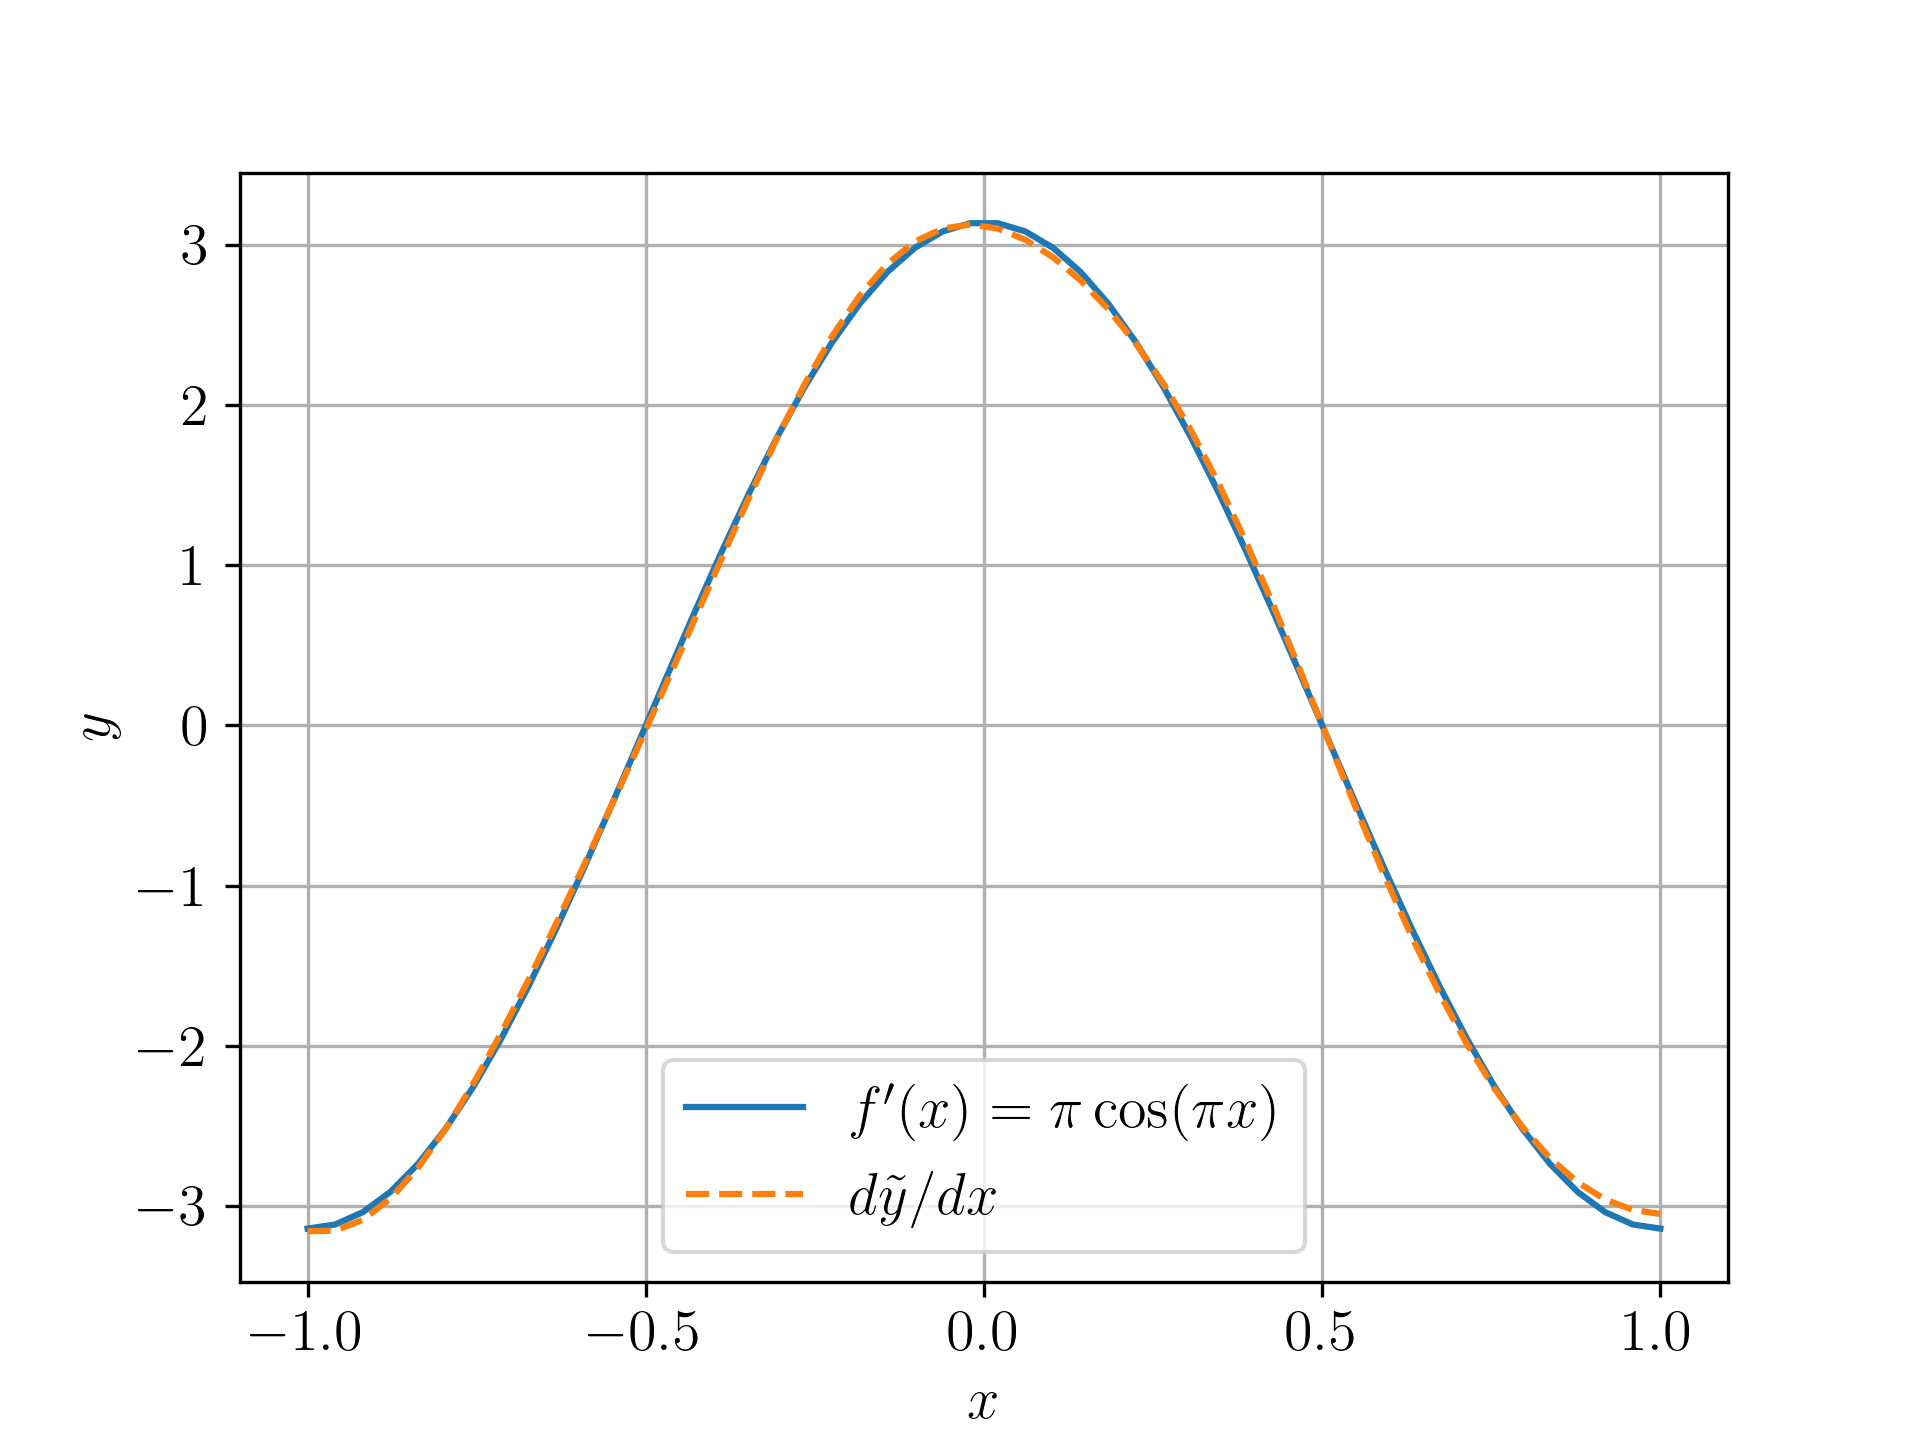
\includegraphics[width=0.8\textwidth]{./cap_mlp/dados/fig_autograd_fun1d/fig}
    \caption{Comparação da autograd da MLP com a derivada exata $f'(x)=\pi\cos(\pi x)$ para o Exemplo \ref{cap_mlp_sec_autograd:ex:fun1d}.}
    \label{cap_mlp_sec_autograd:fig:fun1d}
  \end{figure}

  Uma vez treinada, nossa MLP é uma aproximadora da função seno, i.e. $\tilde{y} \approx \sen(\pi x)$. Usando de autograd podemos computar $\tilde{y}' \approx \pi\cos(\pi x)$. O código abaixo, computa $d\tilde{y}/dx$ a partir da rede e produz o gráfico da figura acima.

\begin{lstlisting}
# verificação
fig = plt.figure()
ax = fig.add_subplot()

xx = torch.linspace(a, b,
                    steps=50).reshape(-1,1)
# y' = cos(x)
dy_esp = torch.pi*torch.cos(torch.pi*xx)
ax.plot(xx, dy_esp, label="$f'(x) = \\pi\cos(\\pi x)$")

# model autograd
dy_est = torch.empty_like(xx)
for i,x in enumerate(xx):
    x.requires_grad = True
    y = model(x)
    y.backward()
    dy_est[i] = x.grad
ax.plot(xx, dy_est, label='$d\\tilde{y}/dx$')

ax.legend()
ax.grid()
ax.set_xlabel('$x$')
ax.set_ylabel('$y$')
plt.show()
\end{lstlisting}
\end{ex}

\subsection{Exercícios}

[[tag:construcao]]
